\section{Physiological Model: Neurovascular Coupling}\label{sec:model}
The \gls{nvc} response, i.e., the ability to locally adjust vascular resistance as a function of neuronal activity, is believed to be mediated by a number of different signaling mechanisms. \citet{Roy1890} first proposed a  mechanism based on a metabolic negative feedback theory. According to this theory, neural activity leads to a drop in oxygen or glucose levels and increases in CO$_2$, adenosine, and lactate levels. All of these signals could dilate arterioles and hence were believed to be part of the neurovascular response. However, recent experiments illustrated that the \gls{nvc} response is partially independent of these metabolic signals \citep{Leithner2010, Lindauer2010, Mintun2001, Powers1996, Makani2010}. An alternative to this theory was proposed where the neuron releases signaling molecules to directly or indirectly affect the blood flow. Many mechanisms such as the \gls{pot} signaling mechanism \cite{Filosa2006}, the \gls{no} signaling mechanism or the arachidonic acid to \gls{eet} pathway are found to contribute to the neurovascular response \citep{Attwell2010}.

The \gls{pot} signaling mechanism of \gls{nvc} seems to be supported by significant evidence, although new evidence shows that the endfoot astrocytic \gls{ca} could play a significant role. The \gls{pot} signaling hypothesis mainly utilises the astrocyte,  positioned to enable the communication between the neurons and the local perfusing blood vessels. The astrocyte and the \glspl{ec} surrounding the perfusing vessel lumen exhibit a striking similarity in ion channel expression and thus can enable control of the \gls{smc} from both the neuronal and blood vessel components \citep{Longden2015}. Whenever there is neuronal activation \gls{pot} ions are released into the \gls{ecs} and \gls{sc}. The astrocyte is depolarised by taking up \gls{pot} released by the neuron and releases it into the \gls{pvs} via the endfeet through the BK channels \citep{Filosa2007}. This increase in \gls{ecs} \gls{pot} concentration ($3-10$ mM) near the arteriole hyperpolarises the \gls{smc} through the \gls{kir} channel, effectively closing the voltage-gated \gls{ca} channel, reducing smooth muscle cytosolic \gls{ca} and thereby causing dilation. Higher \gls{pot} concentrations in the \gls{pvs} cause contraction due to the reverse flux of the \gls{kir} channel \citep{Farr2011}. 

Amidst the difficulty in monitoring and measuring the rapid changes in metabolic demands in the highly heterogeneous brain, speculative estimates of the relative demands of the cerebral processes that require energy were given based on different experimental data by \citet{Ames2000}. As per the estimate, the vegetative processes that maintain the homeostasis including protein synthesis accounted for $10-15$\% of the total energy consumption. The costliest function seems to be in  restoring the ionic gradients during neural activation. The \gls{sodpot} exchange pump is estimated to consume $40-50$\%, while the \gls{ca} influx from organelles and extracellular fluid consumes $3-7$\%. The processing of neurotransmitters such as uptake or synthesis consumes $10-20$\%, while the intracellular signaling systems which includes activation and inactivation of proteins consumes $20-30$\%. The rest of the energy is estimated to be consumed by the axonal and dendritic transport in both directions.

Previous work \cite{Mathias2018} has provided  the construction of an experimentally validated numerical (\textit{in silico}) model based on experimental data to simulate the \gls{fmri} \gls{bold} signal associated with \gls{nvc} along with the associated metabolic and blood volume responses. An existing neuron model \citep{Mathias2017, Mathias2017a} has been extended to include an additional transient \gls{na} ion channel (NaT) expressed in the neuron, and integrated into a complex \gls{nvc} model \citep{Dormanns2015, Dormanns2016, Kenny2017a}. This present model is based on the hypothesis that the \gls{pot} signaling mechanism of \gls{nvc} is the primary contributor to the vascular response and the \gls{sodpot} exchange pump in the neuron is the primary consumer of oxygen during neural activation. The model contains 317 parameters, most of which come from non-human experiments. Based on the work by \cite{Dormanns2016} and \cite{Kenny2018}, we have chosen a subset of parameters defining basic pathways, such as  the nitric oxide and potassium pathways,   that are considered important for the normal function of neurovascular coupling.  We model the uncertainty of the chosen parameters  by representing them as random variables. The remaining  parameters are fixed to nominal values; they include leak terms, characteristic oxygen and other species concentrations, buffer concentrations, volume surface ratios etc\dots By providing random variability to parameters that support these pathways, the dimension of the parameter space is reduced from 317 to 160 which greatly facilitate our analysis. The algorithms defined below can be used to investigate other complex models including that of neurovascular coupling. However for this initial work we constrain ourselves to the above subset. 
Figure \ref{fig:nvu20} shows the components and main pathways of the neurovascular coupling model (version 2.0) \\


\begin{figure}[h!]
\centering
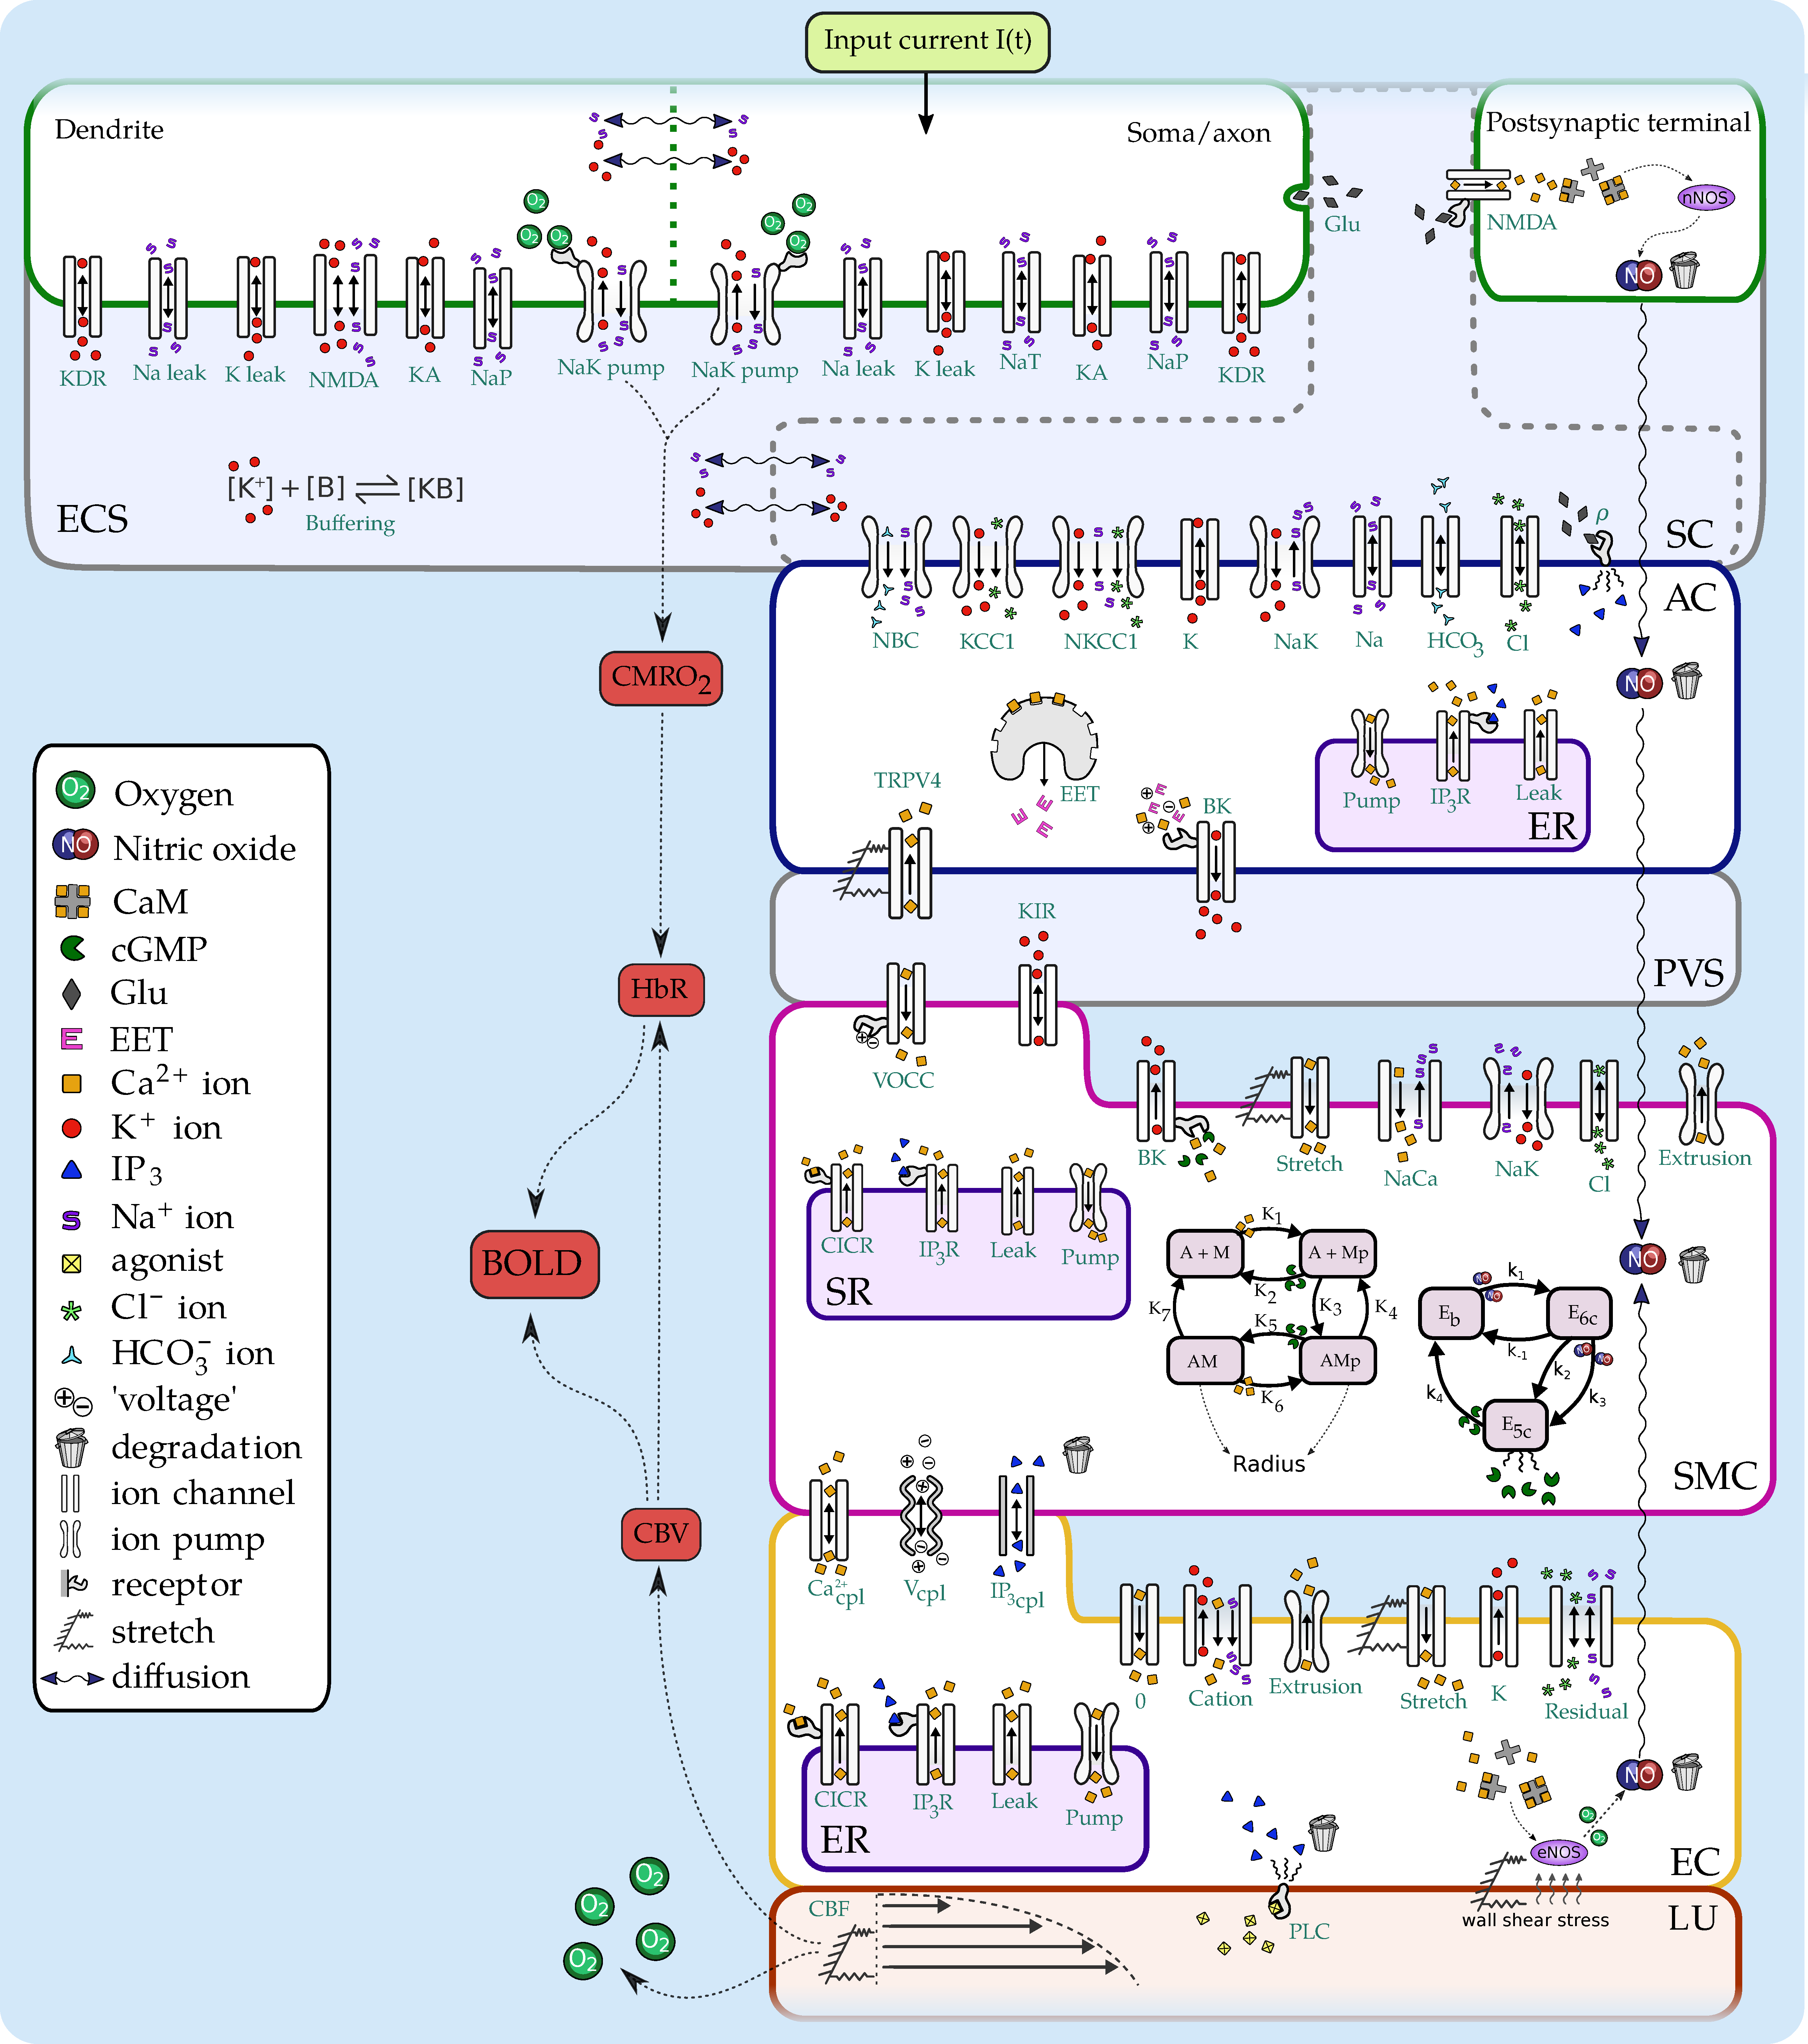
\includegraphics[width=0.7\linewidth]{Figures/nvu_20}
\caption[Graphic Sketch of NVU version 2.0]{Graphic Sketch of NVU version 2.0, showing the basic components of neuron, astrocyte, smooth muscle cell, endothelial cell, lumen and extracellular space. ion channels, pumps and pathways from neuron to endothelial cell are also shown in addition to the basis for evaluation of the fMRI blood oxygenation level signal (BOLD) protocol.}
\label{fig:nvu20}
\end{figure}

  
  
The numerical model outlined in sketch form in Figure \ref{fig:nvu20} is fully defined in the Supplementary Material  and has been developed over a number of years \cite{Farr2011,Dormanns2015,Dormanns2016b}. In order to induce a variation in radius following a neuronal stimulation, an input current is used. The numerical experiments solve equation (\ref{caboodle}) in the presence of short duration electrical (current) stimuli as displayed in Figure~\ref{input_stimuli}. For the presented cases, two input profiles are utilised. Firstly a rectangular pulse of width 10 seconds and magnitude  $I_{max}$ and secondly an experimental pulse sequence used in the work of \cite{Zheng2010} which has the same magnitude as the rectangular pulse but a duration of sixteen seconds followed by second pulse (which is not used in this analysis). Further information about the experiment and the results can be found in \cite{Zheng2010}.  For this second case, the stimulus was a current injection at the whisker pad. This induced an increase in neuronal activity in the somato-sensory cortex which subsequently, through the neurovascular pathway, produced a  change in the radius $R(t)$ allowing increased nutrients to perfuse into the cerebral tissue; this is  the essence of neuro-vascular coupling. 


\begin{figure}[h]
\centering
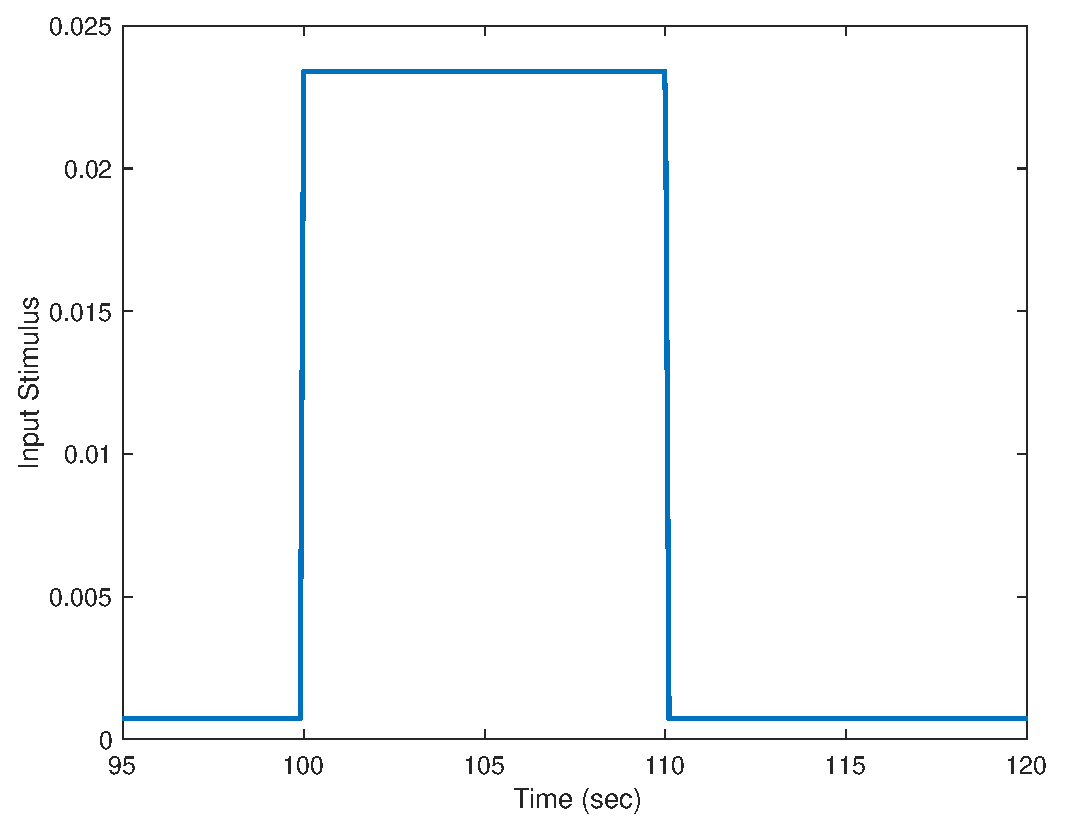
\includegraphics[width=.4 \textwidth]{Figures/Rectangular_Stimulus.eps}
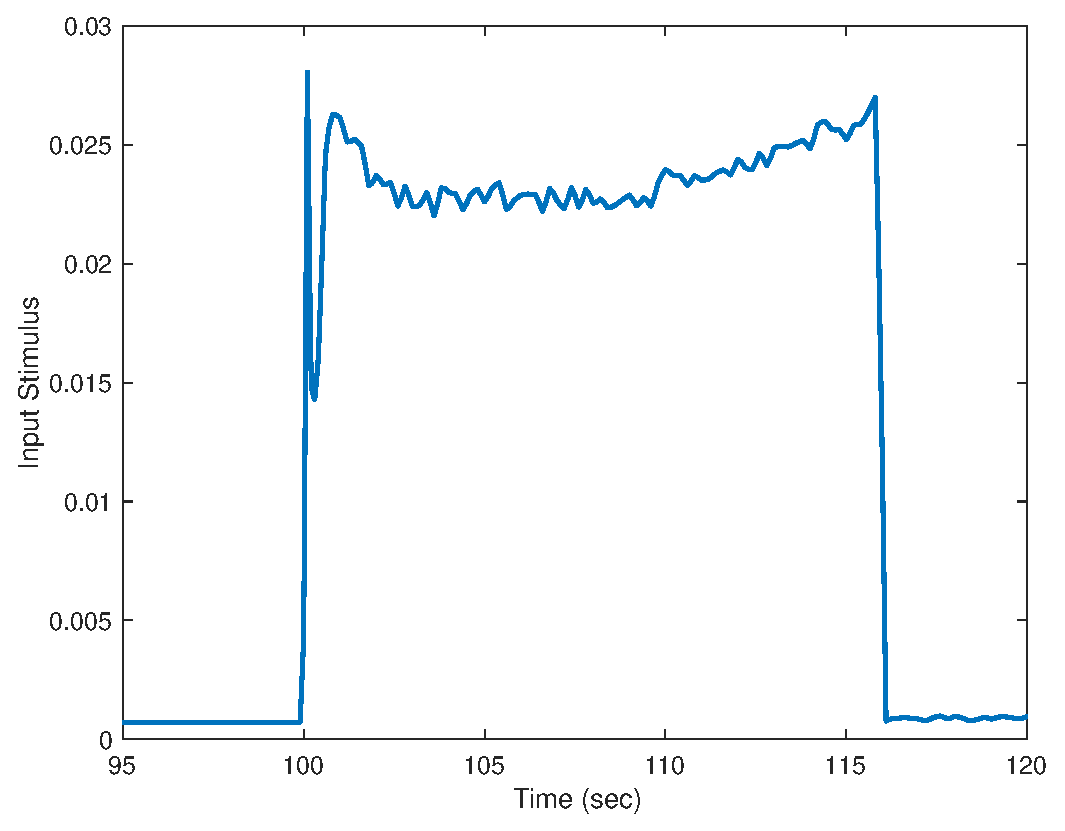
\includegraphics[width=.4 \textwidth]{Figures/Experimental_Stimulus.eps}
\caption{Left: rectangular pulse input stimulus; right: stimulus used in lab experiments.}
\label{input_stimuli}
\end{figure}
  
 We wish to analyse parameter sensitivity of Quantities of Interest (QoIs) that are key to our understanding and quantification of  neurovascular coupling.   From previous work, it is known that the \pot concentration in the extracellular space (ECS) is crucial to maintaining a homeostatic state (large concentrations of \pot support the propagation of spreading depression waves) hence we choose to look at the mean value of \pot in the ECS as our first QoI $q_1$. Secondly, neurovascular coupling is the main phenomenon providing oxygen and nutrients to the neuronal tissue. This is mediated by the local arteriole dilating and (under the assumption of constant pressure) increasing the flow of blood into the tissue. We therefore define the time averaged cerebral blood flow determined over the course of neuronal stimulation as our second QoI, $q_2$. The contraction/dilation of the arteriolar vessel  depends on the smooth muscle cell (SMC) concentration of \ca and the phophorylation of the actin/myocin complex. Our third QoI $q_3$ is the minimum combined concentration of the actin myosin complex, both phosphorylated and unphosphorylated. This allows us to analyse the functioning of the main components of the neurovascular unit (NVU) defined as the linked components of neuron, synaptic ceft, astrocyte, perivascular space (PVS), SMC, endothelial cell (EC), lumen (LU, the domain in which blood flows) and the ECS. 
  Assuming the stimulation occurs for time $t$ between $t_1$ and $t_2$, $t_2>t_1$,  the QoIs are thus
 \begin{itemize}
\item average ECS potassium 
\begin{eqnarray}
%[K^+]_{max,ECS} \label{K_ECS_Max} \\
 q_1 = \frac{1}{t_2-t_1}\int_{t_1}^{t_2}[K^+]_{ECS}(s)\, ds, \label{K_ECS_Mean}
\end{eqnarray}
\item average volumetric flow rate in the cerebral tissue
\begin{eqnarray}
 q_2 = \frac{1}{t_2-t_1}\int_{t_1}^{t_2}\left(\frac{R(s)}{R_0}\right)^4\, ds, \label{vol_flow}
\end{eqnarray}
 \item minimum combined concentration of the actin myosin complex, both phosphorylated and unphosphorylated
\begin{eqnarray}
q_3 = \min _{t, t_1\le t \le t_2} [AM(t)+AM_p(t)]. \label{AM_AMp_Min}
\end{eqnarray}
\end{itemize}

Other examples of sensitivity analysis studies relevant to the general field of biomedicine include \cite{gsa_pharm,lr_gsa,uqpy,Witthoft2013}.
